\section{Data structure}
\label{Sect:DataStructure}

{\bf Lead author:} Adam

The tracker data structure, a subset of the general MAUS data structure, is shown in figure \ref{Fig:DataStructure}.  The basic unit of the MAUS data structure is the spill, representing the data produced by a single actuation of the MICE target.  All MAUS modules (mappers, reducers, etc.) act on one spill at a time.  The spill is then split into two sides, Monte Carlo data and reconstructed data.  A key rule is that MC data must never be stored on the reconstruction side. Each side has its own event class, representing data corresponding to a single MICE particle trigger event.  The relationship between the spill and the MC and recon event objects is one-to-many. 

\begin{figure}[htb]
    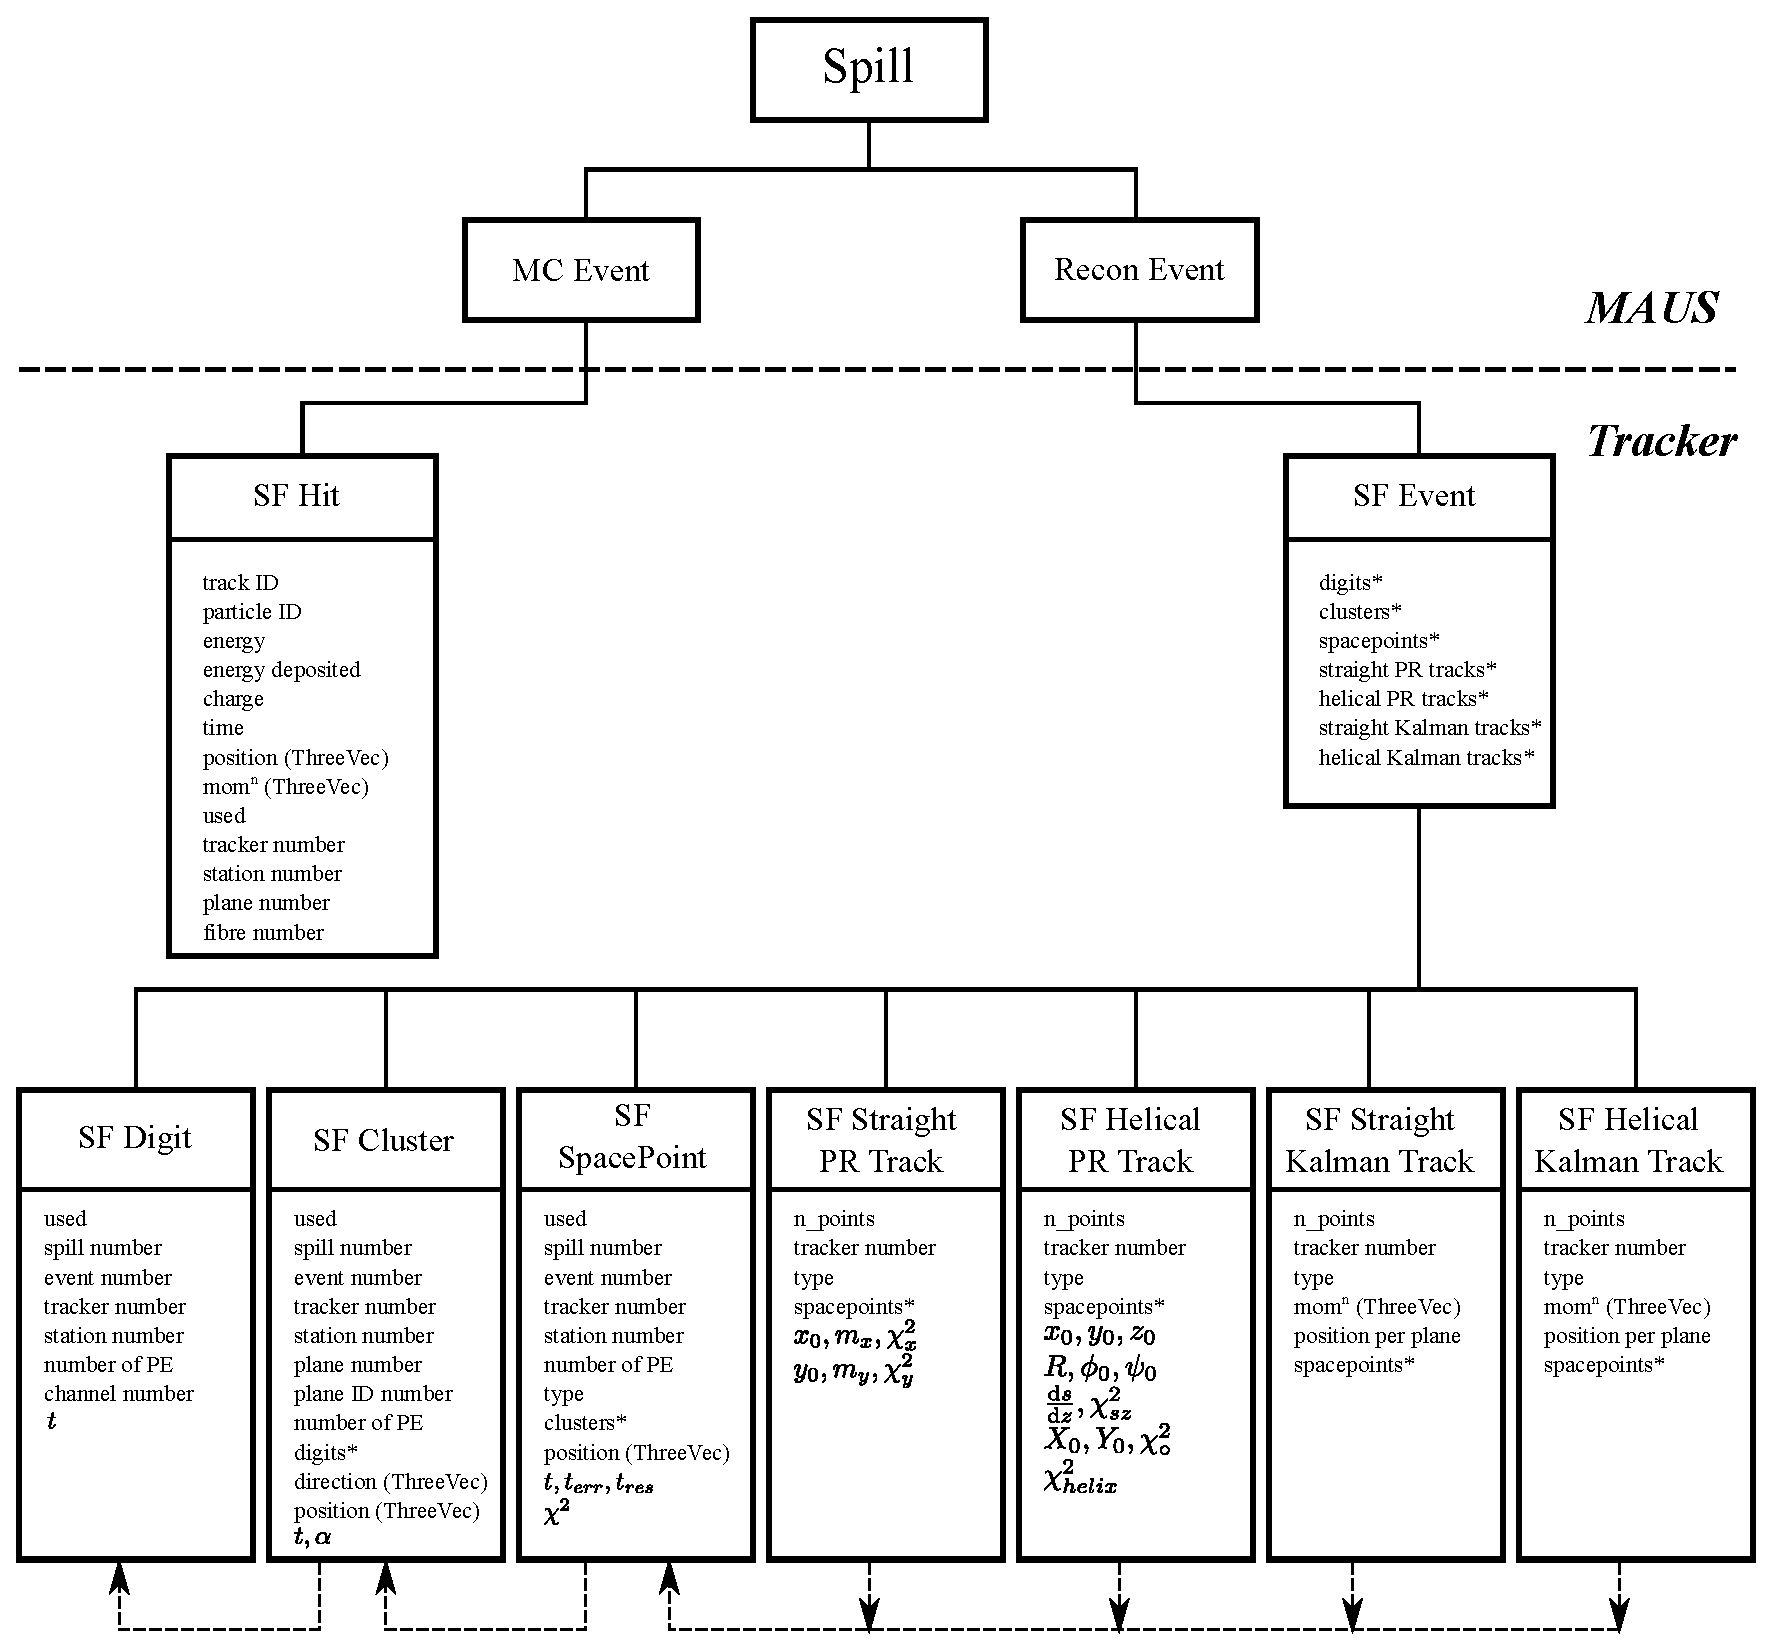
\includegraphics[width=0.85\textwidth]
      {05-DataStructure/Figures/DataStructure.eps}
    \caption{The tracker data structure and its position within the general MAUS data structure.}
    \label{Fig:DataStructure}
\end{figure}

Within an MC event the only data object pertaining to the tracker is the SciFiHit, implemented as template class of the generic Hit class.  This class stores the MC data used by the reconstruction to form SciFiDigits (via the map MapCppTrackerMCDigitisation).  The relationship between MC events and SciFiHits is one-to-many.

On the real data side each recon event holds a single SciFiEvent (a one-to-one relationship). The SciFiEvent then holds a collection (implemented as C++ standard vectors of pointers) for each data type used in the reconstruction process: SciFiDigits, SciFiClusters, SciFiSpacePoints, SciFiStraightPRTracks, SciFiHelicalPRTracks, SciFiStraightKalmanTracks, and  SciFiHelicalKalmanTracks.


